\documentclass{article}%
\usepackage[T1]{fontenc}%
\usepackage[utf8]{inputenc}%
\usepackage{lmodern}%
\usepackage{textcomp}%
\usepackage{lastpage}%
\usepackage[head=40pt,margin=0.5in,bottom=0.6in]{geometry}%
\usepackage{graphicx}%
%
\title{\textbf{Protestaron frente a la ULA para exigir respeto por autonomía universitaria}}%
\author{El Nacional Web}%
\date{05/12/2018}%
%
\begin{document}%
\normalsize%
\maketitle%
\textbf{URL: }%
http://www.el{-}nacional.com/noticias/protestas/protestaron{-}frente{-}ula{-}para{-}exigir{-}respeto{-}por{-}autonomia{-}universitaria\_262204\newline%
%
\textbf{Periodico: }%
EN, %
ID: %
262204, %
Seccion: %
Protestas\newline%
%
\textbf{Palabras Claves: }%
Mérida, Protestas, Sociedad\newline%
%
\textbf{Derecho: }%
2.2%
, Otros Derechos: %
NO\_TIENE%
, Sub Derechos: %
2.2.1%
\newline%
%
\textbf{EP: }%
SI\newline%
\newline%
%
\textbf{\textit{Un grupo de personas encapuchadas cerró la avenida Don Tulio de la entidad}}%
\newline%
\newline%
%
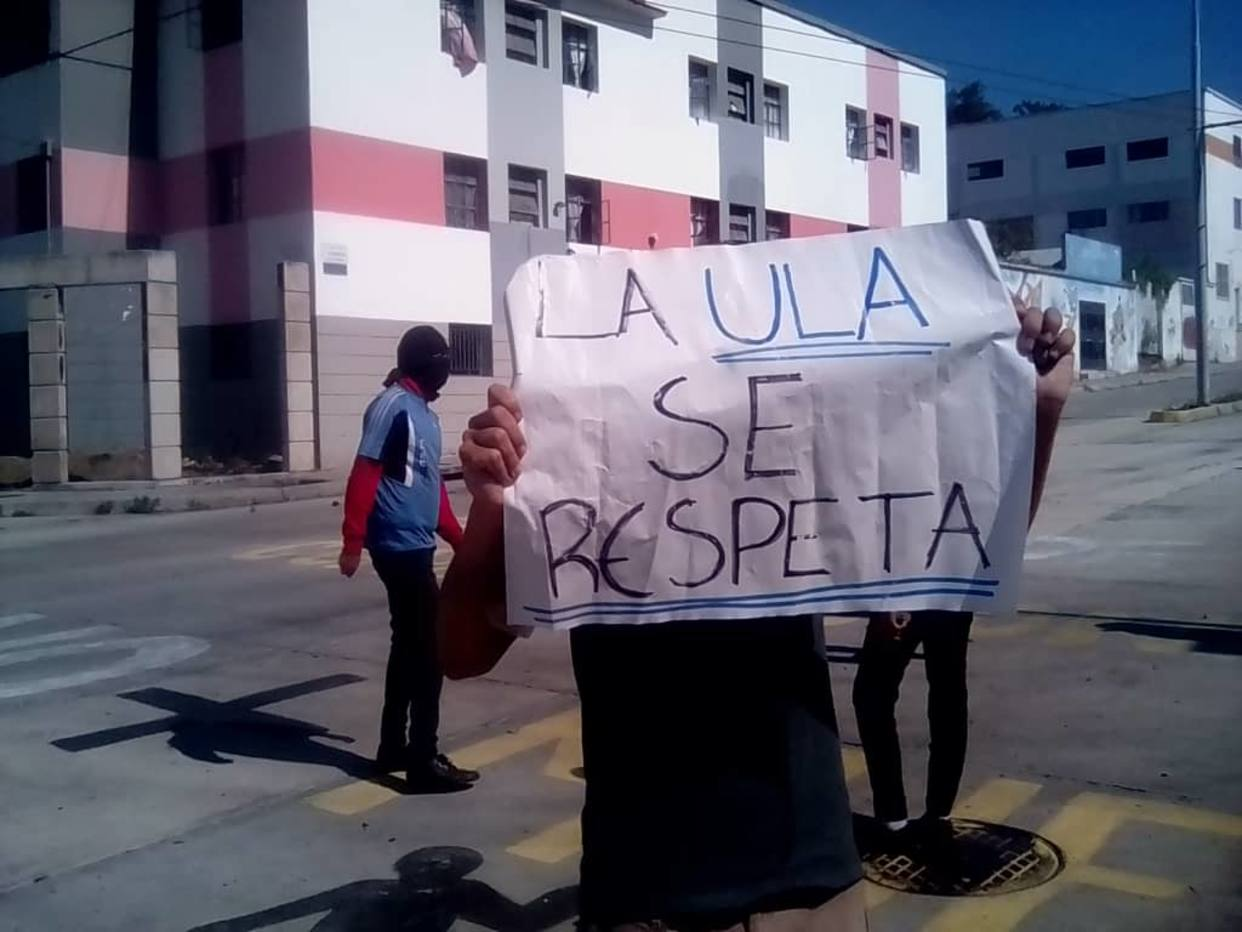
\includegraphics[width=300px]{33.jpg}%
\newline%
%
Un grupo de personas encapuchadas cerró la avenida Don Tulio, ubicada en el estado Mérida, para exigir respeto por la autonomía universitaria.%
\newline%
%
Leonardo León,~El corresponsal de~El Nacional~en la entidad, informó que la protesta se desarrolla frente a la Facultad de Medicina de la Universidad de Los Andes.%
\newline%
%
En las imágenes difundidas por el periodista vía Twitter se puede observar un caucho en proceso de combustión mientras algunas personas sostienen pancartas con mensajes alusivos a su protesta.%
\newline%
%
“La ULA se respeta”, se puede leer en uno de los carteles.%
\newline%
%
\end{document}